% !TeX root = main.tex

\setlength{\abovedisplayskip}{7pt}
\setlength{\belowdisplayskip}{7pt}
\setlength{\abovedisplayshortskip}{4pt}
\setlength{\belowdisplayshortskip}{4pt}

\tableofcontents
\newpage

\section{Система 1}

Рассмотрим систему
\begin{equation}
  \begin{cases}
    \dot x_1=x_2+\sin x_1+x_1^2,\\
    \dot x_2=x_1^2+(2+\sin x_1)u
  \end{cases}
\end{equation}
Для $V(x_1)=\tfrac12x_1^2$ выберем виртуальное управление
\begin{equation}
  x_2=\phi(x_1)=-x_1-\sin x_1-x_1^2
\end{equation}
Тогда $\dot x_1=-x_1$ и $\dot V=-x_1^2$. Введём ошибку
$z_2=x_2-\phi(x_1)$ и составную функцию Ляпунова
\begin{equation}
  V_c=\frac{x_1^2+z_2^2}{2},\qquad
  \dot x_1=-x_1+z_2,\qquad
  \dot z_2=x_1^2+(2+\sin x_1)u-\dot\phi
\end{equation}
Её производная равна
\begin{equation}
  \dot V_c=-x_1^2+
  z_2\bigl[x_1+x_1^2+(2+\sin x_1)u-\dot\phi\bigr]
\end{equation}
По методу бэкстеппинга выбираем
\begin{equation}
  u=\frac{\dot\phi-x_1^2-x_1-z_2}{2+\sin x_1},\qquad
  \dot\phi=(-1-\cos x_1-2x_1)(x_2+\sin x_1+x_1^2)
\end{equation}
Тогда $\dot z_2=-x_1-z_2$ и
\begin{equation}
  \dot V_c=-x_1^2-z_2^2<0\qquad \text{при }(x_1,z_2)\ne(0,0)
\end{equation}
Поскольку $2+\sin x_1\ge1$, управление определено во всём
$\mathbb R^2$. Замена $(x_1,x_2)\mapsto(x_1,z_2)$ глобально обратима,
а $V_c$ радиально неограниченна. Поэтому начало координат глобально
асимптотически устойчиво.

Моделирование выполнено методом Рунге-Кутты четвёртого порядка
с шагом $0{,}001\,\text{с}$ при $\bm x(0)=(1;-0{,}5)^T$,
$t\in[0,10]\,\text{с}$. На рисунке~\ref{fig:system1} состояния
и управление стремятся к нулю.
\begin{figure}[htbp]
  \centering
  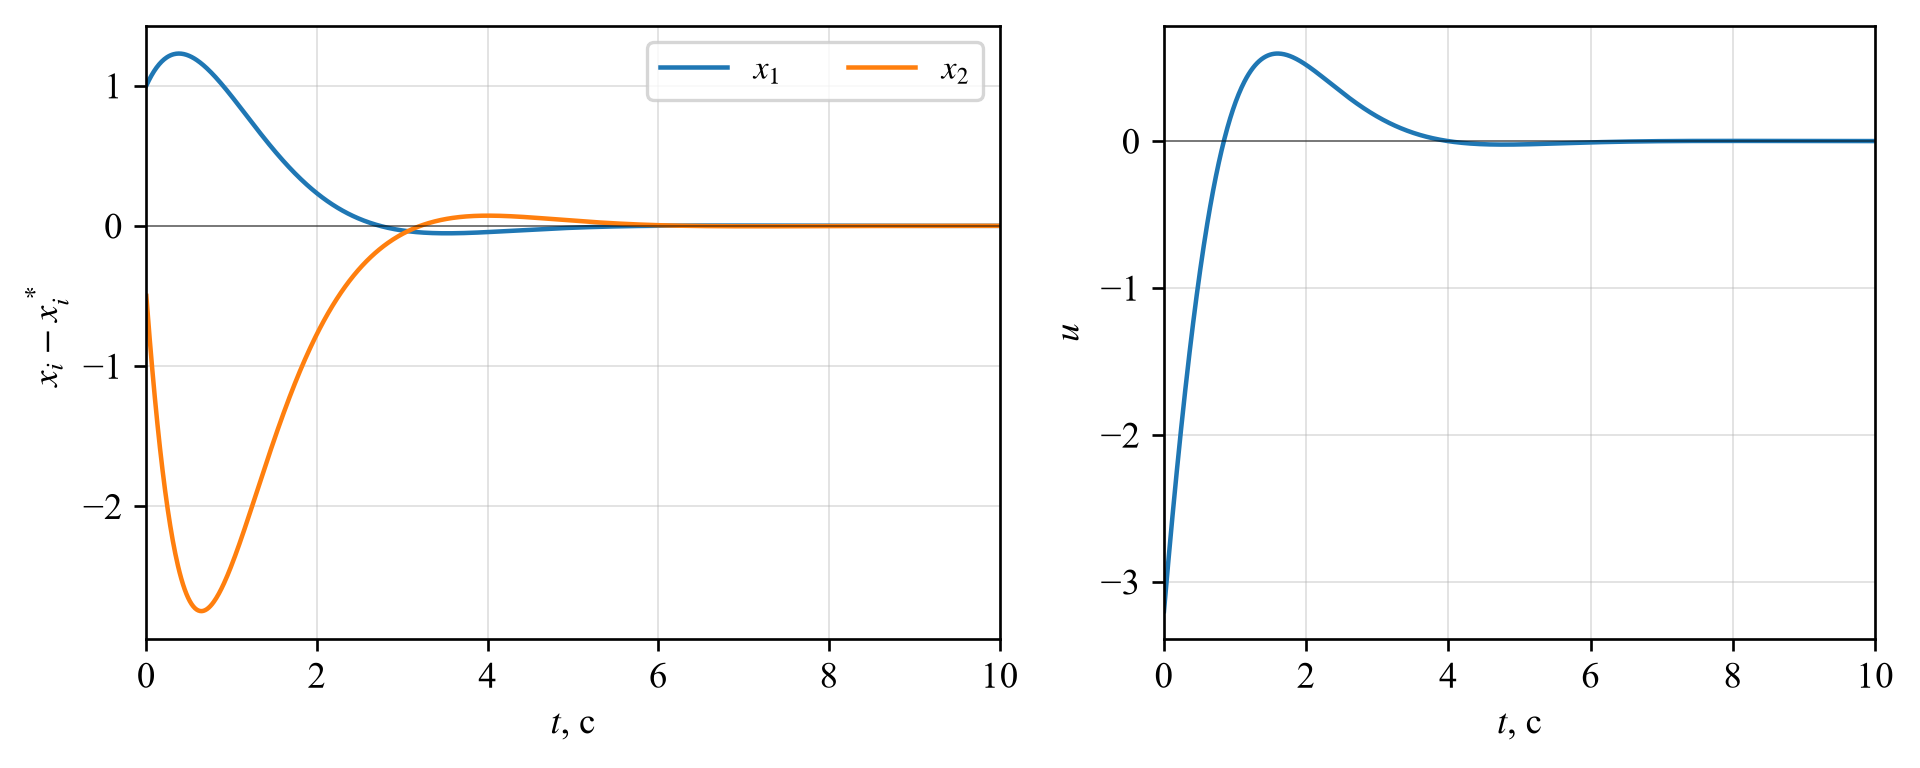
\includegraphics[width=\textwidth]{system1.png}
  \caption{Состояния и управление системы 1}
  \label{fig:system1}
\end{figure}

\clearpage
\section{Система 2}

Рассмотрим систему
\begin{equation}
  \begin{cases}
    \dot x_1=x_2-x_1^3,\\
    \dot x_2=x_1+u
  \end{cases}
\end{equation}
Для $V(x_1)=\tfrac12x_1^2$ выберем $x_2=\phi(x_1)=-x_1$.
Тогда $\dot x_1=-x_1-x_1^3$, $\dot V=-x_1^2-x_1^4$.
В координатах $z_2=x_2+x_1$ имеем
\begin{equation}
  \dot x_1=-x_1-x_1^3+z_2,\qquad
  \dot z_2=u-x_1^3+z_2
\end{equation}
Для составной функции Ляпунова получаем
\begin{equation}
  V_c=\frac{x_1^2+z_2^2}{2},\qquad
  \dot V_c=-x_1^2-x_1^4+z_2(x_1+u-x_1^3+z_2)
\end{equation}
Выбирая управление
\begin{equation}
  u=x_1^3-x_1-2z_2=x_1^3-3x_1-2x_2
\end{equation}
получаем $\dot z_2=-x_1-z_2$ и
\begin{equation}
  \dot V_c=-x_1^2-x_1^4-z_2^2<0\qquad
  \text{при }(x_1,z_2)\ne(0,0)
\end{equation}
Замена координат глобально обратима, а $V_c$ радиально неограниченна.
Следовательно, начало координат глобально асимптотически устойчиво.

Моделирование проведено при $\bm x(0)=(1;-0{,}5)^T$ на интервале
$t\in[0,10]\,\text{с}$. Состояния и управление стремятся к нулю
(рисунок~\ref{fig:system2}).
\begin{figure}[htbp]
  \centering
  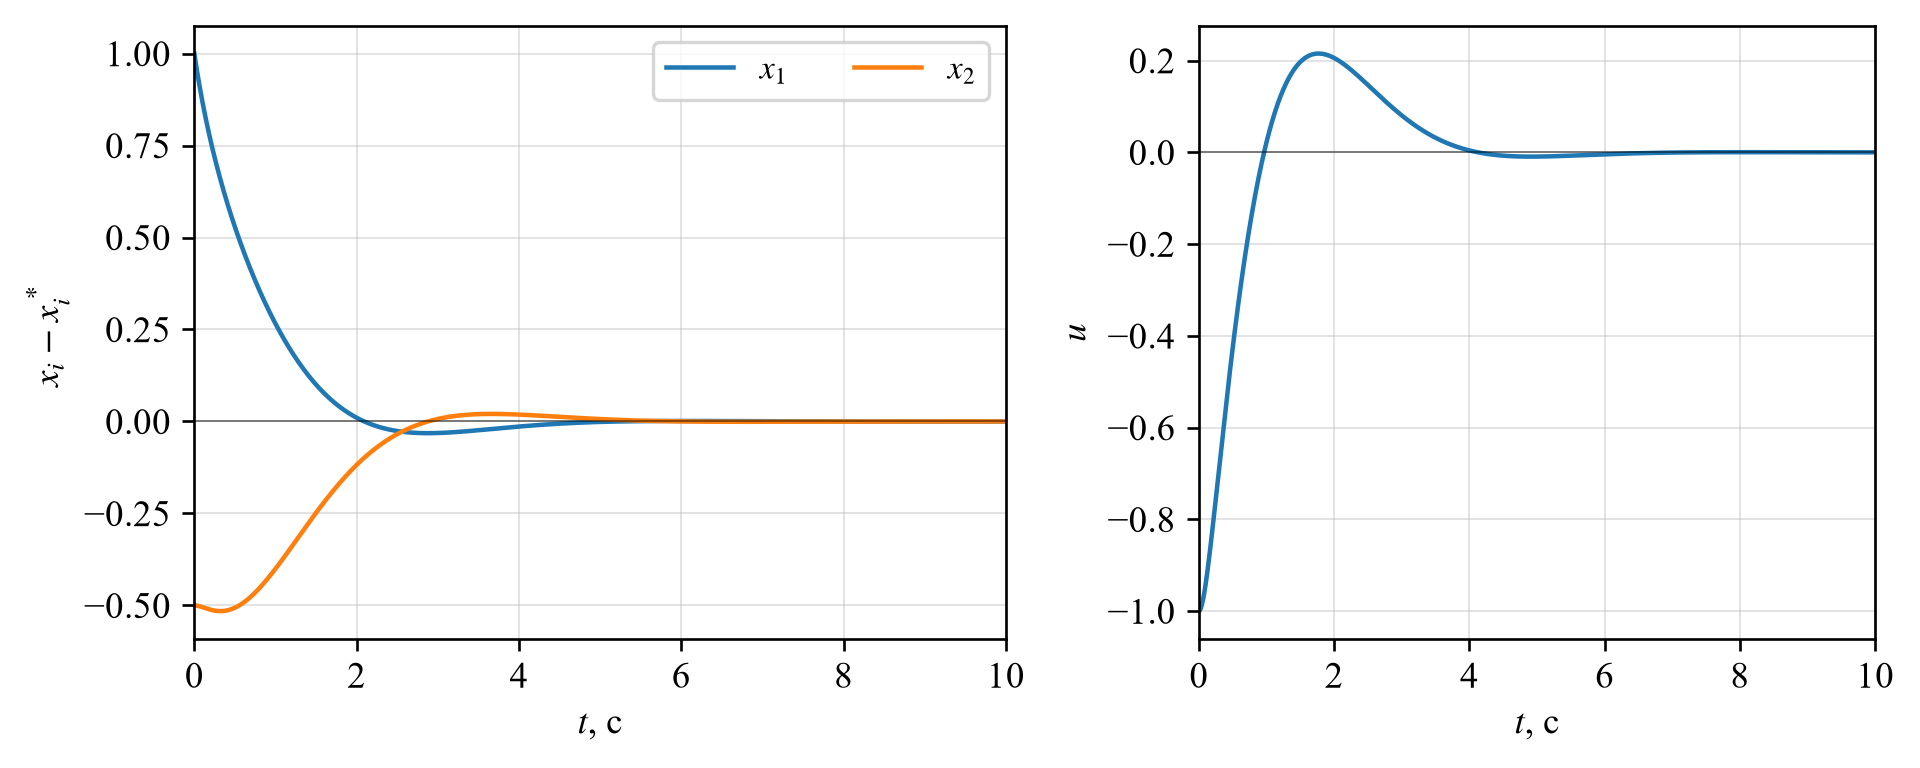
\includegraphics[width=\textwidth]{system2.png}
  \caption{Состояния и управление системы 2}
  \label{fig:system2}
\end{figure}

\clearpage
\section{Система 3}

Рассмотрим систему
\begin{equation}
  \begin{cases}
    \dot x_1=\cos x_1-x_2,\\
    \dot x_2=x_1+x_3,\\
    \dot x_3=x_1x_3+(2-\sin x_3)x_4,\\
    \dot x_4=x_2x_3+2u
  \end{cases}
\end{equation}
Поскольку при $\bm x=0$ имеем $\dot x_1=1$, стабилизируем
равновесие $\bm x^*=(0,1,0,0)^T$, $u^*=0$.

Для $V_1=\tfrac12x_1^2$ выберем виртуальное управление
\begin{equation}
  x_2=\phi_1(x_1)=\cos x_1+x_1,\qquad
  z_2=x_2-\phi_1,\qquad \dot x_1=-x_1-z_2
\end{equation}
При $z_2=0$ получаем $\dot V_1=-x_1^2$.
Для $V_2=V_1+\tfrac12z_2^2$ имеем
\begin{equation}
  \dot z_2=x_1+x_3-\dot\phi_1,\qquad
  \dot V_2=-x_1^2+z_2(x_3-\dot\phi_1)
\end{equation}
Следующий шаг бэкстеппинга задаётся выражениями
\begin{equation}
  \begin{gathered}
    x_3=\phi_2(x_1,x_2)=\dot\phi_1-z_2,\qquad
    \dot\phi_1=(1-\sin x_1)(\cos x_1-x_2),\\
    z_3=x_3-\phi_2,\qquad
    \dot z_2=x_1-z_2+z_3,\qquad
    \dot V_2=-x_1^2-z_2^2+z_2z_3
  \end{gathered}
\end{equation}
Обозначим $g_2(x_3)=2-\sin x_3\ge1$.
Для $V_3=V_2+\tfrac12z_3^2$ получаем
\begin{equation}
  \dot V_3=-x_1^2-z_2^2+
    z_3\bigl[z_2+x_1x_3+g_2x_4-\dot\phi_2\bigr]
\end{equation}
Выберем третье виртуальное управление
\begin{equation}
  x_4=\phi_3(x_1,x_2,x_3)
      =\frac{\dot\phi_2-x_1x_3-z_2-z_3}{g_2},\qquad
  z_4=x_4-\phi_3
\end{equation}
Тогда $\dot z_3=-z_2-z_3+g_2z_4$.
Производные виртуальных управлений вычисляются по исходной системе:
\begin{equation}
  \dot\phi_i=\sum_{j=1}^{i}
       \frac{\partial\phi_i}{\partial x_j}\dot x_j,
  \qquad i=2,3
\end{equation}
Они не содержат $u$, поэтому итоговый закон является обратной
связью по состоянию:
\begin{equation}
  u=\frac12\bigl(\dot\phi_3-x_2x_3-g_2z_3-z_4\bigr)
\end{equation}
Он обеспечивает $\dot z_4=-g_2z_3-z_4$. Для полной функции Ляпунова
имеем
\begin{equation}
  V_c=\frac{x_1^2+z_2^2+z_3^2+z_4^2}{2},\qquad
  \dot V_c=-x_1^2-z_2^2-z_3^2-z_4^2
\end{equation}
Все функции гладкие во всём $\mathbb R^4$, поскольку $g_2\ge1$.
Треугольная замена $(x_1,x_2,x_3,x_4)\mapsto(x_1,z_2,z_3,z_4)$
глобально обратима и переводит $\bm x^*$ в нуль.
Функция $V_c$ радиально неограниченна, а её производная отрицательно
определена. Следовательно, равновесие $\bm x^*$ глобально
асимптотически устойчиво.

\begin{samepage}
Моделирование проведено при
$\bm x(0)=(0{,}5;1;-0{,}5;0{,}25)^T$ на интервале
$t\in[0,10]\,\text{с}$. На рисунке~\ref{fig:system3} показаны
отклонения $\bm x-\bm x^*$ и управление. Отклонения и управление
стремятся к нулю.
\par
\end{samepage}
\begin{figure}[htbp]
  \centering
  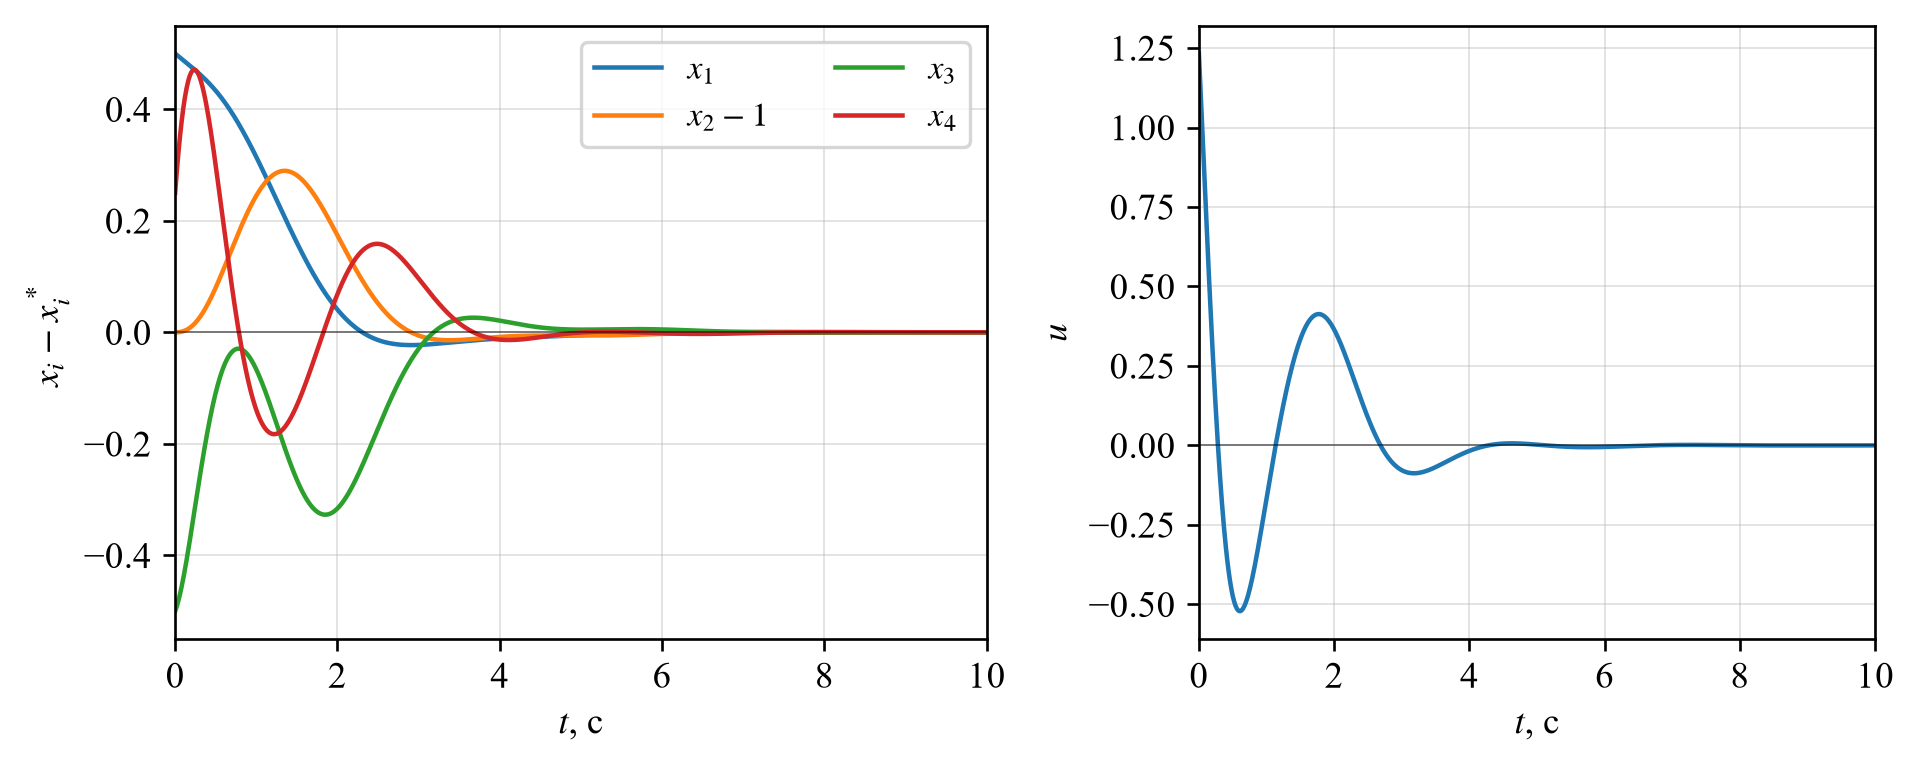
\includegraphics[width=\textwidth]{system3.png}
  \caption{Отклонения состояний и управление системы 3}
  \label{fig:system3}
\end{figure}
